\documentclass[systems,article,submit,pdftex,moreauthors]{Definitions/mdpi}

% Official MDPI submission class. Publication details are assigned by MDPI.
\firstpage{1}
\makeatletter
\setcounter{page}{\@firstpage}
\makeatother
\pubvolume{1}
\issuenum{1}
\articlenumber{0}
\pubyear{2026}
\copyrightyear{2026}
\datereceived{ }
\daterevised{ }
\dateaccepted{ }
\datepublished{ }
\hreflink{}
% Reserve enough space for the MDPI review header with current fancyhdr.
\geometry{headheight=25pt}
% Submission copies do not yet have an assigned citation or DOI.
\renewcommand{\leftcolUpdateCitation}{}
\makeatletter
\apptocmd{\ps@plain}{\fancyfoot[R]{}}{}{\ClassError{mdpi}{Cannot clear the unassigned DOI footer}{}}
\makeatother

\usepackage{listings}
\usetikzlibrary{arrows.meta,positioning}
\lstset{basicstyle=\scriptsize\ttfamily, breaklines=true, frame=single, framerule=0.3pt,
  captionpos=b, aboveskip=6pt, belowskip=2pt, xleftmargin=2pt, xrightmargin=2pt,
  breakindent=0pt, abovecaptionskip=2pt, columns=fullflexible, keepspaces=true}

\Title{Seeing the Process Through the Worker's Eyes: Event Logs from Egocentric Factory Videos}
\TitleCitation{Seeing the Process Through the Worker's Eyes: Event Logs from Egocentric Factory Videos}
\newcommand{\orcidauthorA}{0000-0002-3279-4795}
\newcommand{\orcidauthorB}{0000-0002-0955-6940}
\Author{Alessandro Berti $^{1,}$*\orcidA{} and Wil M. P. van der Aalst $^{1,2}$\orcidB{}}
\AuthorNames{Alessandro Berti and Wil M. P. van der Aalst}
\AuthorCitation{Berti, A.; van der Aalst, W.M.P.}
\address{%
$^{1}$ \quad Process and Data Science (PADS), RWTH Aachen University, Aachen, Germany;\\
\hspace*{1.1em} a.berti@pads.rwth-aachen.de (A.B.); wvdaalst@pads.rwth-aachen.de (W.M.P.v.d.A.)\\
$^{2}$ \quad Celonis, Munich, Germany}
\corres{Correspondence: a.berti@pads.rwth-aachen.de}

\abstract{Process mining usually relies on event logs from information systems, which often miss manual work on factory shop floors. Egocentric video captures this work but must be converted into structured events. We present a five-stage pipeline that uses foundation models to describe videos, create a shared vocabulary for each factory, and extract events with consistent labels and estimated timestamps. The pipeline requires no task-specific training or human annotation. Applied to six factories in Egocentric-10K, it produces 322 event logs with 10{,}698 events from 59 workers. We assess log structure, agreement with transcripts, and the analyses the logs support. All events follow the required schema and vocabularies. A small manual audit gives event precision of 0.86 against the transcripts. The logs quantify work-time composition, interruptions, and differences among workers performing the same dominant process. They identify a 10.8\% rework share in one factory and suggest different priorities for material presentation and logistics. Missing vocabulary labels, limited waiting coverage, and incomplete extraction from long recordings restrict the conclusions. The pipeline, prompts, derived data, and assessment code are public.}
\keyword{process mining; event log extraction; egocentric video; large language models; manufacturing; process improvement; decision support}

\begin{document}

\section{Introduction}
\label{sec:introduction}

Process mining uses event logs to study how operational processes work. An event log contains timestamped activity records grouped into cases~\cite{vanDerAalst2016processmining}. This approach depends on digital records of the work. Many manual tasks on a factory shop floor leave no such records. Picking a part from a bin, loading a blank into a die, and moving material between stations may be absent from the information system. A manufacturing execution system may record order or machine checkpoints, while the sequence, duration, and interruptions of manual work remain unknown~\cite{kratsch2022video}.

Egocentric video offers another source of evidence. Head-mounted cameras record work from the worker's perspective. They capture hand movements, interactions with tools and objects, and movement between stations. The Egocentric-10K corpus\footnote{\url{https://huggingface.co/datasets/builddotai/Egocentric-10K}} contains thousands of hours of factory footage (Figure~\ref{fig:egocentric}). However, video must be converted into events before process mining can use it. Each event needs a consistent activity label, timestamps, and a case identifier. Creating these records by hand takes considerable effort.

\begin{figure}[t]
\centering
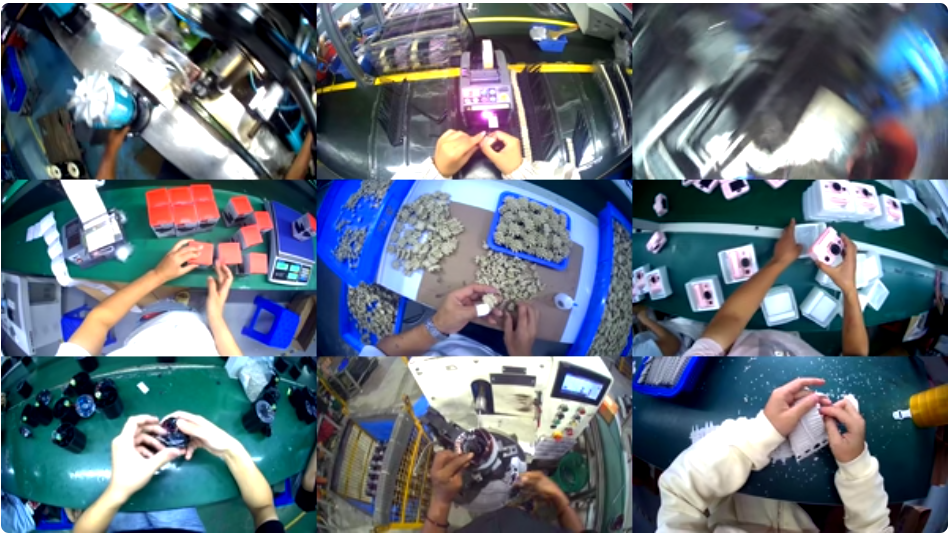
\includegraphics[width=0.88\linewidth]{figures/egocentric10k.png}
\caption{Frames from Egocentric-10K (Build AI), showing manual factory work from the worker's perspective. Source: the public dataset linked in the text (Apache License 2.0).}
\label{fig:egocentric}
\end{figure}

Three lines of research address parts of this problem (Section~\ref{sec:relatedWork}). Video-based process mining often uses fixed cameras and vision models built for a specific setting. Sensor-based process mining converts signals with less descriptive detail into events. Work on large language models (LLMs) extracts event logs from text. Applying these methods to egocentric video also requires event segmentation, timestamp estimation, and consistent labels across recordings.

We present a five-stage pipeline that converts egocentric factory video into event logs using foundation models. Applied to six factories from Egocentric-10K, it produces 322 per-video logs with 10{,}698 events from 59 workers. These logs are inferred observations and require validation before use. We address three research questions.
\textbf{RQ1 (Feasibility and validity):} Can the pipeline produce structurally valid event logs for hundreds of videos without task-specific training or human annotation?
\textbf{RQ2 (Fidelity):} How well do the extracted events match the transcripts in timing and meaning?
\textbf{RQ3 (Value):} Which operational analyses and improvement decisions do the logs support, and what are their limits?
Our contributions are the pipeline and its design choices, a public derived dataset for six factories,\footnote{\url{https://github.com/fit-alessandro-berti/annotated-egocentric-10k-dataset}} an assessment of log validity and analytical value, and an account of the main limitations. The study connects manual work, information systems, and process improvement by making work that is usually unrecorded available for analysis.

\section{Related Work}
\label{sec:relatedWork}

\emph{Event log construction and data quality.} Building an event log involves extraction, correlation, and abstraction~\cite{diba2020extraction}. Choosing what counts as a case is part of this process. Inferred logs can contain uncertain timestamps, unclear event boundaries, and missing events. These risks motivate the validity checks in this study.

\emph{Process mining on video data.} Knoch et al.~\cite{knoch2020video} extracted traces from fixed-camera recordings of manual assembly without labeled training data. Kratsch et al.~\cite{kratsch2022video} proposed a reference architecture that combines video preprocessing, activity recognition, and event abstraction. Lepsien et al.~\cite{lepsien2023analytics} developed a pipeline with activity recognition and event correlation. SnapLog~\cite{pegoraro2026snaplog} uses image embeddings, temporal segmentation, and a few labeled example frames to extract events. Sensor-based process mining provides related methods for converting lower-level signals into events~\cite{brzychczy2025sensor}.

Our approach differs in four ways. First, the camera follows the worker across stations and records detailed interactions with objects. Second, the pipeline uses general-purpose foundation models without task-specific training or labeled examples. Third, it creates a shared vocabulary of readable process and activity labels for each factory. Fourth, the assessment considers both extraction quality and the operational questions that the resulting logs can answer.

\emph{LLM-assisted process mining.} Previous work benchmarks LLMs on process mining tasks~\cite{berti2025benchmark} and uses them to extract event logs from text~\cite{dani2025llm}. We use video as the original source. Timestamped transcripts provide the basis for event boundaries, while controlled vocabularies keep labels consistent across recordings.

\section{Materials and Methods}
\label{sec:approach}

The pipeline (Figure~\ref{fig:pipeline}) converts video into event logs in five automated stages. It follows two design choices. First, it describes the video before assigning process mining labels. Labels are introduced after a factory vocabulary has been created~\cite{diba2020extraction}. Second, event extraction uses only labels from that vocabulary. This reduces inconsistent labels across videos and workers, although it cannot guarantee that an event is correct. The pipeline uses no fine-tuning or human annotation. All prompts are publicly available.

\begin{figure}[t]
\centering
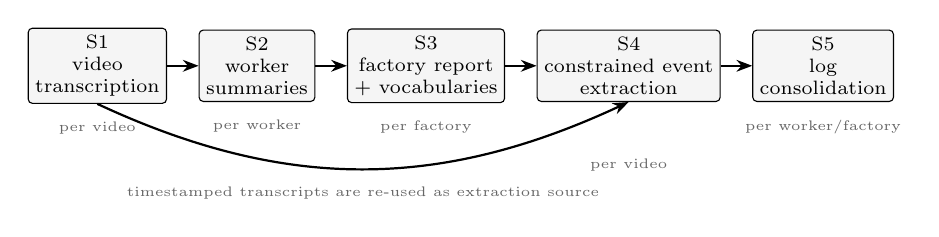
\begin{tikzpicture}[
  node distance=3mm and 4mm,
  stage/.style={draw, rounded corners=1.5pt, align=center, font=\scriptsize, inner sep=2.5pt, minimum height=7.5mm, fill=black!4},
  art/.style={align=center, font=\tiny, text=black!60},
  arr/.style={-{Stealth[length=2mm]}, thick}
]
\node[stage] (s1) {S1\\video\\transcription};
\node[stage, right=of s1] (s2) {S2\\worker\\summaries};
\node[stage, right=of s2] (s3) {S3\\factory report\\+ vocabularies};
\node[stage, right=of s3] (s4) {S4\\constrained event\\extraction};
\node[stage, right=of s4] (s5) {S5\\log\\consolidation};
\draw[arr] (s1) -- (s2);
\draw[arr] (s2) -- (s3);
\draw[arr] (s3) -- (s4);
\draw[arr] (s4) -- (s5);
\draw[arr] (s1.south) to[out=-25, in=-155] node[art, below, yshift=-1mm]{timestamped transcripts are re-used as extraction source} (s4.south);
\node[art, below=1mm of s1] {per video};
\node[art, below=1mm of s2] {per worker};
\node[art, below=1mm of s3] {per factory};
\node[art, below=6mm of s4] {per video};
\node[art, below=1mm of s5] {per worker/factory};
\end{tikzpicture}
\caption{The five-stage pipeline: a multimodal model (S1 to S3) produces transcripts, summaries, and vocabularies; a text-only model (S4) converts each transcript into vocabulary-constrained events; S5 consolidates CSV logs.}
\label{fig:pipeline}
\end{figure}

\subsection{Source data}
We processed videos from six factories in Egocentric-10K, covering 59 workers and 322 clips. Table~\ref{tab:proc} describes the work in each factory. The selected clips are usually about 20 minutes long, while a few recordings span several hours.

\begin{table}[t]
\centering
\caption{Domain and dominant processes per factory. Process labels stem from the induced S3 vocabularies; percentages are shares of observed event time.}
\label{tab:proc}
\footnotesize
\setlength{\tabcolsep}{4pt}
\begin{tabularx}{\linewidth}{@{}l>{\raggedright\arraybackslash}p{0.30\linewidth}L@{}}
\toprule
Factory & Domain & Dominant processes (time share) \\
\midrule
001 & Metal hardware stamping and bench assembly & Metal stamping (48\%), manual mechanical assembly (34\%), component bagging (7\%) \\
002 & Garment finishing and packaging & Fabric folding (19\%), garment bagging (17\%), garment ironing (13\%) \\
003 & Investment-casting post-processing & Surface finishing and polishing (42\%), wax pattern assembly (19\%), defect patching (11\%) \\
004 & Garment sewing and confection & Overlock seaming (24\%), garment folding (11\%), thread trimming (11\%) \\
005 & Machining and electric motor assembly & Manual lathe machining (32\%), drill press machining (19\%), material transport and logistics (10\%) \\
006 & Sand-casting foundry & Sand mold creation (17\%), pattern cleaning and coating (14\%), compression molding (12\%) \\
\bottomrule
\end{tabularx}
\end{table}

\subsection{S1: Change-point transcription}
In S1, a multimodal model (Gemini~3.1 Pro) produces a chronological description of each video (Listing~\ref{lst:s1}). The prompt asks for a new timestamped entry when the action, object, location, focus of attention, or social context changes. Repeated work is kept in one interval while it remains unchanged. These boundaries later guide event extraction. The prompt also asks the model to describe what is visible without imposing process labels and to state uncertainty when scenes are unclear. S1 produced 13{,}304 timestamped entries for the 322 videos.

\begin{lstlisting}[caption={Extract of the S1 video transcription prompt.},label={lst:s1},float=t]
Please transcribe the attached egocentric video into a very detailed chronological text description. [...] Format every entry as: [HH:MM:SS - HH:MM:SS] description [...] Only create a new entry when something meaningful changes, such as: the action changes / a new object is handled / the person changes location [...] If a repeated behavior continues in exactly the same way, summarize that repeated stretch once [...] If the scene is partially unclear, mention the uncertainty briefly instead of guessing. Do not use tables, bullets, JSON, labels, categories, or analysis language.
\end{lstlisting}

\subsection{S2 and S3: Summaries and vocabularies}
S2 combines each worker's transcripts into a report with a process summary, a detailed breakdown, possible improvements, and evidence limits. Suggestions concern process design and exclude judgments about individual workers. S3 combines the worker reports for a factory and creates two controlled vocabularies: 12 to 24 process labels and 55 to 131 activity labels per factory. A process label describes a broad task, such as \emph{metal stamping}. An activity label uses a verb-object phrase, such as \emph{load raw metal blank into die}. The prompt asks for labels covering transport, staging, waiting, setup, cleanup, inspection, and handoffs, as well as the main production tasks. It also asks the model to avoid near-duplicate labels. Listings~\ref{lst:s2} and~\ref{lst:s3} show the main instructions. The two vocabularies allow analysis at process and activity levels.

\begin{lstlisting}[caption={Extract of the S2 worker summarization prompt.},label={lst:s2},float=t]
You are given multiple detailed chronological transcriptions from egocentric factory videos recorded by the same worker. Your task is to synthesize those transcriptions into a process-focused report [...] Only suggest process optimizations that are visible or reasonably inferable from the observed workflow. [...] Do not suggest worker-level optimizations such as "work faster" [...] Write plain text with exactly these section headings: Process Summary / Detailed Process Breakdown / Possible Process Optimizations / Evidence Limits
\end{lstlisting}

\begin{lstlisting}[caption={Extract of the S3 vocabulary induction prompt.},label={lst:s3},float=t]
Produce a long, detailed, process-mining-oriented activity catalogue for the factory [...] Each activity must be a short string only, suitable as a candidate event label for process mining. Prefer specific verb-object phrases such as "load raw blank into press" rather than generic labels such as "operate machine". Include not only value-adding operations, but also transport, staging, waiting, inspection, rework-like handling, setup, cleanup, handoff, documentation, and coordination activities when visible. [...]
\end{lstlisting}

\subsection{S4: Constrained event extraction}
In S4, a text-only LLM (GPT-5.4) converts each transcript into a JSON event list. Each event has an estimated start time, an estimated end time, an activity, and a process. Both labels must come from the factory vocabularies. Transcript timestamps provide the main basis for event boundaries. An interval with one stable activity becomes one event, while an interval containing several activities may be split. The prompt excludes non-work segments and permits an empty event list. The parser checks the output schema and vocabulary membership (Listing~\ref{lst:s4}). For example, a transcript entry from 00:04:05 to 00:04:36 describes placing a frame, pouring powder, and scraping the surface. One extracted event covers 00:04:24 to 00:04:36 with activity \emph{level powder surface with wooden scraper} and process \emph{Sand mold creation}.

\begin{lstlisting}[caption={Extract of the S4 constrained event extraction prompt.},label={lst:s4},float=t]
You are converting one timestamped raw factory annotation into a structured event list for process mining. [...] The value of `activity` must be exactly one label from the allowed factory activity list; the value of `process` exactly one label from the allowed factory process list. Do not invent new labels. [...] If multiple labels are plausible, choose the closest allowed label. [...] Each array item must be an object with exactly these keys: `estimated_start_time`, `estimated_end_time`, `activity`, `process` [...] Include only process-relevant operational events. [...] If no valid operational events can be extracted, return {"events":[]}.
\end{lstlisting}

\subsection{S5: Log consolidation}
S5 merges the per-video CSV files into worker and factory logs. Each event records its start and end time, activity, process, factory, and worker. Clips from one worker are joined in recording order on a synthetic timeline starting at 2000-01-01. The videos have no wall-clock metadata, so the timeline preserves durations and ordering rather than real calendar dates. Merged events include a source file, a \texttt{case\_id}, time offsets, and durations. The same data can support different case definitions, including a video, a worker, or a process phase. Our assessment uses a video as a case.

\subsection{Design rationale}
The text representation separates video interpretation from event labeling. Transcripts are created once and can be inspected, reused for vocabulary creation, and checked against extracted events. Each factory has its own vocabulary because the work differs by domain. Broader process labels provide an additional level of abstraction for analysis.
\section{Results}
\label{sec:assessment}

We assess the inferred logs in three steps. \textbf{Q1 (Validity):} Do the logs meet structural checks, and how well do they match the transcripts? \textbf{Q2 (Analysis capability):} Which process mining analyses can use them, and what do those analyses show? \textbf{Q3 (Improvement evidence):} Do the logs add useful evidence to the qualitative reports produced by the pipeline? The computations use pm4py~\cite{berti2023pm4py} and the released artifacts. The assessment code is public and does not require access to model APIs.

\subsection{Q1: Validity Preconditions}
Table~\ref{tab:corpus} reports the corpus and validity checks. All 10{,}698 events contain the required fields, are in chronological order, and use labels from the factory vocabularies. Between 89\% and 97\% of activity labels are used. For the 314 recordings up to one hour, median event coverage is about 95\%. The seven multi-hour recordings have a median coverage of 1.2\% because extraction stops early. Recordings longer than one hour are excluded from the time statistics below. About 82\% of event boundaries fall within 5\,s of a transcript boundary. One author checked a stratified sample of 42 events and 42 transcript entries. Strict event precision was 0.86, no labels contradicted the transcripts, and operational recall was about 0.89. \textbf{Finding F1:} The logs pass the structural checks and show useful agreement with the transcripts for shorter recordings. These checks do not measure errors in the initial video interpretation.

\begin{table}[t]
\centering
\caption{Corpus and validity preconditions (Q1) per factory. Conf.\ = share of event labels in the factory vocabularies; Cov.\ = share of observed span covered by events; Align.\ = share of event boundaries within $\pm$5\,s of a transcript boundary.}
\label{tab:corpus}
\footnotesize
\setlength{\tabcolsep}{3.5pt}
\begin{tabular}{@{}lrrrrrrrrrr@{}}
\toprule
Factory & Workers & Videos & Events & \multicolumn{2}{c}{Activity vocab.} & \multicolumn{2}{c}{Process vocab.} & Conf. & Cov. & Align. \\
\cmidrule(lr){5-6}\cmidrule(lr){7-8}
 & & & & size & used & size & used & & & \\
\midrule
001 & 11 & 97 & 2{,}288 & 131 & 125 & 13 & 13 & 100\% & 94.8\% & 93.1\% \\
002 & 10 & 54 & 1{,}541 & 75 & 67 & 24 & 24 & 100\% & 28.2\% & 71.8\% \\
003 & 11 & 72 & 2{,}449 & 55 & 52 & 12 & 12 & 100\% & 93.0\% & 86.8\% \\
004 & 10 & 51 & 1{,}893 & 71 & 65 & 22 & 22 & 100\% & 92.1\% & 90.4\% \\
005 & 11 & 22 & 1{,}103 & 102 & 97 & 18 & 17 & 100\% & 25.0\% & 75.0\% \\
006 & 6 & 26 & 1{,}424 & 61 & 59 & 24 & 24 & 100\% & 14.1\% & 62.1\% \\
\midrule
All & 59 & 322 & 10{,}698 & & & & & 100\% & 52.8\% & 82.1\% \\
\bottomrule
\end{tabular}
\end{table}

\subsection{Q2: Analysis Capability}
We apply four analyses: work-time composition (A1), interruptions (A2), process flow (A3), and worker comparison (A4). For A1 and A2, the 112 process labels are mapped to seven categories: value-adding transformation (VA), material handling and staging (MH), transport (TR), quality inspection (QI), cleaning and maintenance (CM), rework (RW), and documentation (DOC). This mapping groups process labels by their operational role. It is released with the assessment code.

\subsubsection{A1: Work-time composition.}
Table~\ref{tab:value} reports how event-covered time is divided among operational categories. The share outside value-adding work ranges from 3.7\% to 25.8\%. Factory 006, a foundry, spends about one quarter of this time on handling, transport, and cleaning. In factory 003, \emph{Defect patching} accounts for \textbf{10.8\% of event-covered time}. This suggests that casting quality deserves further investigation. Factory 005 has the highest transport share, at 9.7\%. \textbf{Finding F2:} The logs quantify how recorded manual work time is spent, including a rework share that the qualitative reports did not identify.

\begin{table}[t]
\centering
\caption{Value analyses per factory (recordings over one hour excluded). Left (A1): share of event-covered time per operational category. Right (A2): median value-adding (VA) share per worker, interruptions of VA work per hour, and median uninterrupted VA run.}
\label{tab:value}
\footnotesize
\setlength{\tabcolsep}{3.4pt}
\begin{tabular}{@{}lrrrrrrr@{\hspace{4mm}}rrr@{}}
\toprule
 & \multicolumn{7}{c}{A1: time composition} & \multicolumn{3}{c}{A2: fragmentation} \\
\cmidrule(lr){2-8}\cmidrule(l){9-11}
Factory & VA & MH & TR & QI & CM & RW & DOC & VA share & Intr./h & VA run \\
\midrule
001 & 93.1 & 4.1 & 1.8 & 0.0 & 0.2 & 0.0 & 0.9 & 94.5\% & 9.2 & 4.6 min \\
002 & 96.3 & 0.1 & 2.3 & 0.2 & 0.0 & 0.0 & 1.1 & 97.3\% & 3.9 & 8.8 min \\
003 & 82.1 & 0.4 & 0.0 & 0.0 & 6.3 & \textbf{10.8} & 0.4 & 86.4\% & 3.6 & 9.0 min \\
004 & 89.9 & 3.0 & 3.5 & 2.0 & 0.9 & 0.0 & 0.7 & 91.3\% & 10.6 & 3.6 min \\
005 & 80.6 & 5.4 & 9.7 & 4.3 & 0.0 & 0.0 & 0.0 & 85.9\% & 5.6 & 6.2 min \\
006 & 74.2 & \textbf{12.1} & 7.8 & 0.0 & 5.7 & 0.0 & 0.3 & 87.0\% & \textbf{14.4} & \textbf{3.1 min} \\
\bottomrule
\end{tabular}
\end{table}

\subsubsection{A2: Fragmentation of value-adding work.}
Time shares alone do not show how often work is interrupted. Frequent short replenishment trips may require a different response from one long trip with the same total duration. We group consecutive events in the same category into runs for each worker. Table~\ref{tab:value} reports the median worker VA share, interruption frequency, and uninterrupted VA run duration. Factory 001 has 6.9\% non-VA time and 9.2 VA interruptions per hour. Its material handling and transport episodes average 15\,s, which points to material presentation at the workstation as a possible improvement. Factory 006 combines 14.4 VA interruptions per hour with 19.8\% of time in material handling and transport. Its median uninterrupted VA run is 3.1 minutes. This profile suggests a need to examine layout and logistics. \textbf{Finding F3:} Combining time shares and interruption frequency helps identify different process improvement priorities. The data suggest interventions but do not establish their effects.

\subsubsection{A3: Flow visibility.}
We apply Inductive Miner~\cite{leemans2013inductive} with a noise threshold of 0.2 and each video as a case. At activity level, token-based replay fitness ranges from 0.95 to 0.99 and precision from 0.06 to 0.27. Nearly all traces are unique. Workers mix handling and cleaning with production cycles, so a detailed model can become difficult to read. Activity-level logs still support local sequence analysis: self-loops account for 4\% to 17\% of directly-follows pairs. Grouping events by process gives 12 to 24 labels and 2 to 26 segments per trace. In factory 001, process-level precision reaches 0.59 at fitness above 0.96, compared with activity-level precision of 0.069. These results support process-level discovery with activity-level analysis for detail.

\subsubsection{A4: Worker benchmarking.}
A shared factory vocabulary allows workers with the same dominant process to be compared (Table~\ref{tab:bench}). In factory 003, the VA shares of five surface-finishing workers range from 67.3\% to 96.9\%. In factory 004, two ironing workers differ by about 24 percentage points. These differences identify stations or observation windows that deserve closer study. They may reflect workstation design, task mix, or other conditions. The two lathe machinists in factory 005 differ by less than one percentage point, which also motivates examining shared working conditions. Across factories, the three largest VA activities account for 27\% to 62\% of VA time. This helps identify tasks for further tooling or automation analysis. \textbf{Finding F4:} The logs reveal differences of up to 30 percentage points in VA share among workers with the same dominant process. These comparisons generate hypotheses rather than individual performance ratings.

\begin{table}[t]
\centering
\caption{A4: worker benchmarking on shared dominant processes (workers with at least 30 minutes of observed footage).}
\label{tab:bench}
\footnotesize
\begin{tabular}{@{}llrll@{}}
\toprule
Factory & Shared process & Workers & VA share & Mean VA run \\
\midrule
001 & Manual mechanical assembly & 6 & 89.7 to 97.8\% & 1.7 to 6.7 min \\
001 & Metal stamping & 3 & 90.6 to 98.5\% & 3.2 to 7.9 min \\
003 & Surface finishing and polishing & 5 & \textbf{67.3 to 96.9\%} & 3.3 to 13.7 min \\
004 & Garment ironing & 2 & \textbf{52.8 to 77.1\%} & 3.5 to 4.1 min \\
004 & Overlock seaming & 4 & 87.8 to 96.5\% & 1.5 to 10.3 min \\
005 & Manual lathe machining & 2 & 95.0 to 95.8\% & 6.9 to 9.4 min \\
\bottomrule
\end{tabular}
\end{table}

\subsection{Q3: Comparing Improvement Evidence}
The S3 factory reports describe possible improvements without using the event logs. We compare these observations with the log results in Table~\ref{tab:tri}. The comparison shows how logs can quantify a concern, change the suggested response, or reveal a missing label. For example, the short, frequent handling episodes in factory 001 suggest examining material presentation before adding dedicated handlers. In factory 003, the process vocabulary has no transport label even though transport appears in the transcripts. Its low measured transport share therefore cannot be read as evidence that transport is absent. Requiring vocabulary checks for transport, waiting, rework, and inspection would help identify such gaps. \textbf{Finding F5:} Event logs add quantities to narrative observations and can expose both further improvement opportunities and limits in what the vocabulary can represent. Since both outputs come from the same transcripts, their agreement is not independent validation.

\begin{table}[t]
\centering
\caption{Q3: comparison of qualitative report claims with event-log evidence.}
\label{tab:tri}
\footnotesize
\begin{tabularx}{\linewidth}{@{}LLL@{}}
\toprule
Report claim (S3, qualitative) & Log evidence (quantitative) & Relation \\
\midrule
001: ``most pervasive bottleneck is the lack of dedicated material handlers'' & 449 MH/TR episodes, 14.6/h, mean 15\,s, 5.9\% of time & \textbf{Refined}: frequency, not time share; presentation, not headcount \\
006: ``excessive manual material handling ... facility-wide bottleneck'' & 19.8\% of time in MH/TR, 28.4 episodes/h, VA runs of 3.1 min & \textbf{Confirmed, quantified}: largest measured MH/TR time share \\
003: workers ``halt value-adding operations to carry heavy metal trays'' & MH/TR only 0.4\%; the 003 vocabulary has \textbf{no transport label} & \textbf{Blind spot}: transport is transcribed but not representable \\
003 report does not mention rework & \emph{Defect patching} = 10.8\% of observed time & \textbf{New finding}: rework priority for further investigation \\
\bottomrule
\end{tabularx}
\end{table}

\subsection{What the Logs Cannot (Yet) Answer}
The logs have four main limits. First, they lack product identifiers and counts, so they cannot measure throughput or first-pass yield without further object information~\cite{aalst2019objectcentric}. Second, synthetic timestamps do not represent shifts, breaks between recordings, or calendar-time utilization. Third, material is not tracked across workers, so handoff events do not reconstruct a complete factory flow. Fourth, the extraction prompt removes non-operational footage and much waiting time. The logs therefore under-measure waiting.

\section{Discussion}
\label{sec:discussion}

\subsection{Threats to Validity}
The category mapping involves judgment, such as deciding whether mold coating adds value. The mapping is public so that these choices can be examined. Fidelity checks compare events with transcripts rather than video, so errors in video interpretation may remain undetected. A video-based audit is needed before operational decisions. Filtering of waiting and incomplete extraction from long recordings also limit the measured time shares. The semantic audit was conducted by one author on 42 events and 42 transcript entries, with no inter-rater agreement measure. The study covers six factories from one discrete-manufacturing corpus, and results depend on prompts and model versions. Finally, worker comparisons use observation windows of different lengths. They do not establish causes or justify judgments about individuals.

\subsection{Ethical Considerations}
Egocentric video records work from a personal viewpoint. The worker comparisons show why privacy and appropriate use matter~\cite{mannhardt2018privacy}. The pipeline limits improvement suggestions to process design. Released logs use pseudonymous worker identifiers, and the repository does not redistribute source videos. Use in a workplace requires appropriate consent, a clear purpose, aggregation, and access controls. Comparisons should guide investigation of working conditions and workstation design.

\section{Conclusions}
\label{sec:conclusion}

We presented a five-stage pipeline that converts egocentric factory video into event logs without task-specific training or manual annotation. It produced 322 logs with 10{,}698 events from six factories. The assessment shows that the logs support analysis of work-time composition, interruptions, local process patterns, and differences between workers performing the same dominant process. The results include a 10.8\% rework share in one factory and different interruption profiles that suggest different improvement priorities. The logs also have clear limits. They depend on the initial video interpretation and factory vocabularies, omit much waiting, and cover long recordings poorly. Future work should add vocabulary coverage checks, extraction in shorter time windows, video-based audits, real calendar timestamps, and object references. The public pipeline, prompts, derived data, and assessment code provide a basis for testing and extending this approach.

\section*{Declarations}

\authorcontributions{Alessandro Berti carried out the experiments. Wil M. P. van der Aalst reviewed the manuscript and suggested improvements.}

\funding{Funded by the European Union. This work received funding from the European High Performance Computing Joint Undertaking (JU), the German Federal Ministry of Research, Technology and Space (BMFTR), the Ministry of Culture and Science of North Rhine-Westphalia (MKW NRW), and the Hessian Ministry of Science and Research, Arts and Culture (HMWK), under grant agreement No. 101250682.}

\institutionalreview{This study is a secondary analysis of the existing Egocentric-10K dataset. It involved no recruitment of participants, intervention, or new video collection. No ethics approval or exemption record for this secondary analysis is reported.}

\informedconsent{No participants were recruited or contacted for this secondary analysis. The source videos were obtained from the existing Egocentric-10K dataset. The authors did not collect new consent, and the source dataset card does not report the original consent procedure.}

\dataavailability{The pipeline, prompts, transcripts, factory vocabularies, derived event logs, and assessment code are available at \url{https://github.com/fit-alessandro-berti/annotated-egocentric-10k-dataset}. The source videos are available from Build AI's Egocentric-10K dataset at \url{https://huggingface.co/datasets/builddotai/Egocentric-10K}, under its access terms and Apache License 2.0. The repository contains derived artifacts and does not redistribute the source videos.}

\acknowledgments{The study used Gemini 3.1 Pro for video descriptions, worker summaries, and factory reports, and GPT-5.4 for event extraction, as described in the methods. OpenAI Codex (GPT-6) assisted with language editing, LaTeX formatting, and preparation of the cover letter. The authors are responsible for the content of this work.}

\conflictsofinterest{Wil M. P. van der Aalst is affiliated with Celonis, a process mining software company. No other conflicts of interest are reported.}

\begin{adjustwidth}{-\extralength}{0cm}
\reftitle{References}
\bibliography{references}
\end{adjustwidth}

\end{document}
